\documentclass{article}\usepackage[utf8]{inputenc}\usepackage[T1]{fontenc}\usepackage{lmodern}\usepackage{amsmath}\usepackage{tikz}\pagestyle{empty}\begin{document}\begin{center}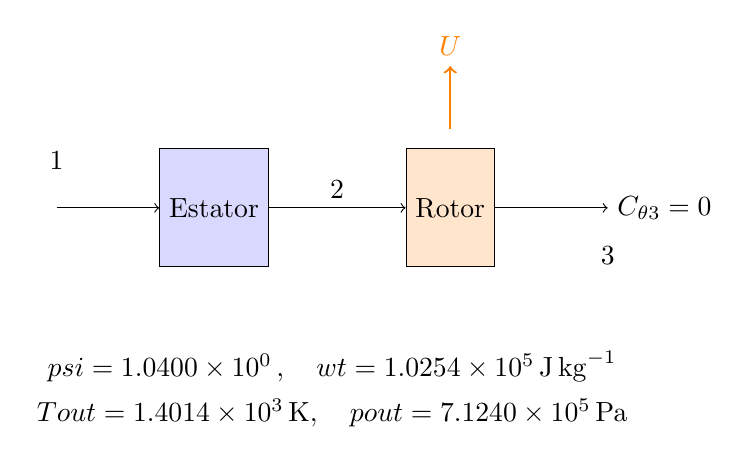
\begin{tikzpicture}\node[draw,fill=blue!15,minimum height=1.5cm] (s) at (2,1) {Estator};\node[draw,fill=orange!20,minimum height=1.5cm] (r) at (5,1) {Rotor};\draw[->] (0,1)--(s);\draw[->] (s)--(r) node[midway,above] {2};\draw[->] (r)--(7,1) node[right] {$C_{\theta3}=0$};\node at (0,1.6) {1};\node at (7,.4) {3};\draw[->,orange,thick] (5,2)--(5,2.8) node[above] {$U$};\node[below,align=center] at (3.5,-0.7) {$psi=1.0400\times10^{0}\,,\quad wt=1.0254\times10^{5}\,\mathrm{J}\,\mathrm{kg}^{-1}$};\node[below,align=center] at (3.5,-1.2999999999999998) {$Tout=1.4014\times10^{3}\,\mathrm{K},\quad pout=7.1240\times10^{5}\,\mathrm{Pa}$};\end{tikzpicture}\end{center}\end{document}